\chapter{Analysis of Parasite Clearance Times}
\section{Comparison of PC90 by experimental factors}
The derived PC90 values using the log-linear interpolation method are shown in Table \ref{derivedPC90}
\begin{table}[h]
\centering
\caption{Derived PC90 values in hours}\label{derivedPC90}
\begin{tabular}{|cc|c|c|}
\hline
&&\multicolumn{2}{c|}{Treatment}\\
&&alone&combined\\\hline
\multirow{2}{*}{Centre 1}&Male&$\begin{array}{c}3.85,\ 27.32,\ 36.30,\  8.84,\\4.35,\  1.53,\ 30.01,\  4.83\end{array}$&$\begin{array}{c}9.47,\  5.05,\  8.10,\\22.77,\  9.40,\  7.73\end{array}$\\\cline{2-4}
&Female&$\begin{array}{c}19.76,\ 22.45,\\21.75,\ 46.52\end{array}$&$\begin{array}{c}3.65,\ 8.40 ,\ 9.69,\\0.85,\ 9.04,\ 9.38\end{array}$\\\hline
\multirow{2}{*}{Centre 2}&Male&$\begin{array}{c}4.82,\ 2.21,\\11.59,\ 28.09\end{array}$&$\begin{array}{c}17.15,\ 9.51,\\14.68,\ 8.08\end{array}$\\\cline{2-4}
&Female&$\begin{array}{c}21.97,\ 2.49,\ 25.08,\ 31.63,\\5.00,\ 21.64,\ 24.42\end{array}$&$\begin{array}{c}14.77,\  8.75,\\5.84,\ 6.23\end{array}$\\\hline
\end{tabular}
\end{table}
\subsection{Graphical comparison}
The PC90 data from Table \ref{derivedPC90} are plotted by experimental factors centre, sex and treatment in Figure \ref{pc90boxes}, summarised in two ways. Firstly, by the median and upper and lower quartiles. Secondly, the mean is shown with 95\% confidence intervals from the $t$ distribution defined by the standard error of the data\footnote{The $t$ distribution confidence intervals are calculated using the \texttt{smean.cl.normal} \emph{R} functions from the Hmisc library\cite{Hmisc}}. These confidence intervals for the mean are relevant for parametric tests based on the normal distribution such as ANOVA and give an indication of differences that may be significant.
\begin{figure}[h]
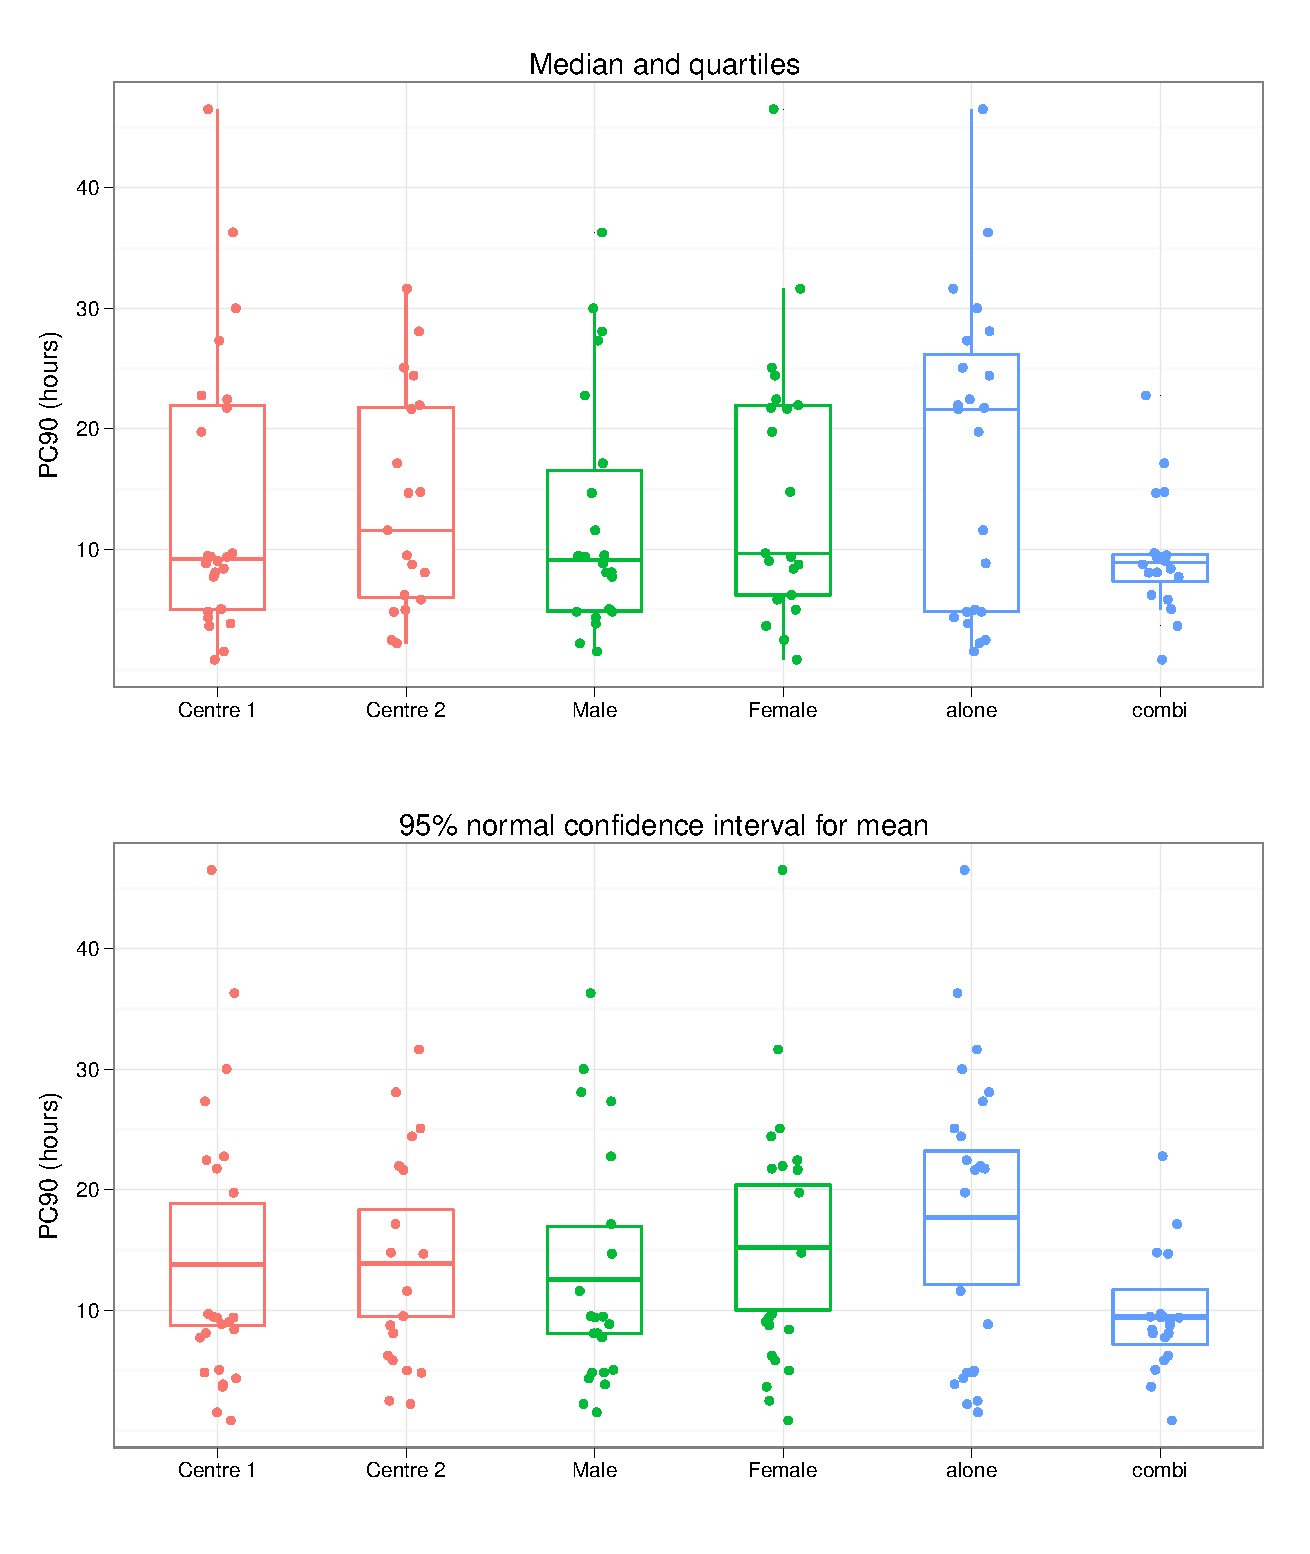
\includegraphics[width=6.5in]{pc90boxes.eps} 
\caption{Comparison of PC90 by experimental factors with medians and quartiles and $t$ distribution 95\% confidence intervals for the means}
\label{pc90boxes}
\end{figure}

It can be seen in Figure \ref{pc90boxes} that there doesn't seem to be any notable difference in clearance times between centres. Female subjects seem to have a larger variance in clearance times and perhaps a slightly longer clearance time on average. The difference in clearance times due to the treatment chosen seems to have the largest influence with a larger spread in clearance times for subjects on the ``alone'' single-drug treatment with a potentially significant decrease in mean clearance time for the subjects on the combined-drug treatment.

An additional observation is that the distributions seem bimodal in the cases of the Centre 1, Female and alone subjects. LOOK AT RAW PLOTS TO SEE WHAT IS GOING ON.

In Figure \ref{pc90interaction} the data is split two ways in each plot to look for interaction effects betwee the factors. Again, the mean and 95\% confidence intervals for the mean are shown.
\begin{figure}[ht]
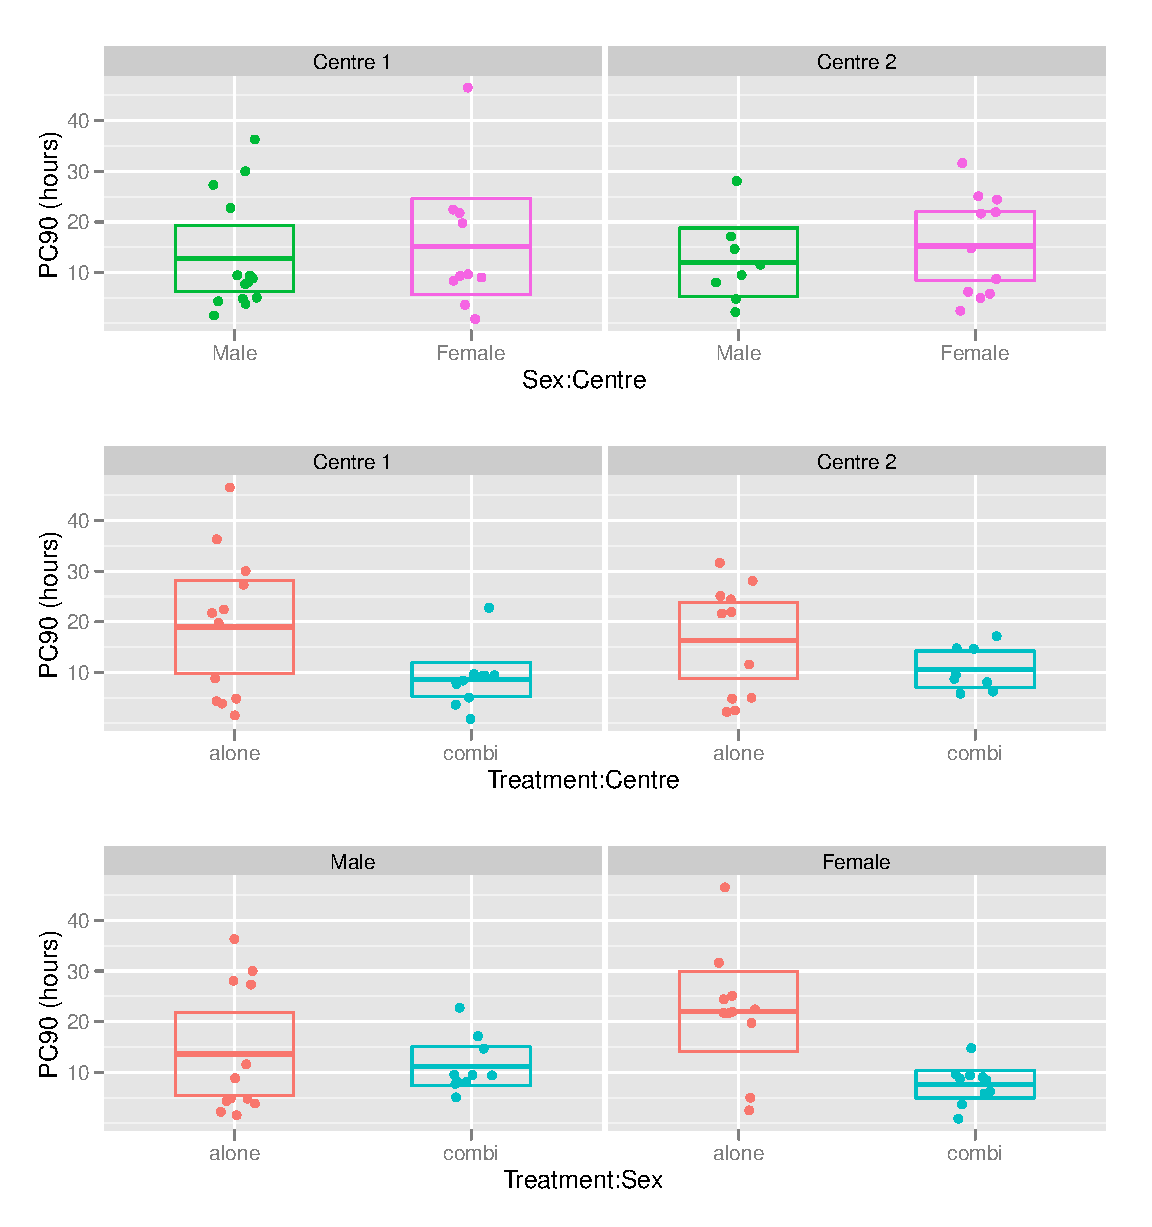
\includegraphics[width=6.5in]{pc90interaction.eps} 
\caption{PC90 two-way interactions with 95\% confidence intervals for the means}
\label{pc90interaction}
\end{figure}

It can be seen that there doesn't seem to be any interaction between sex and centre or treatment and centre i.e. the left and right panels of the top two plots look essentially the same. However, it appears that the combined treatment only decreases the mean clearance time for female subjects.
\subsection{Statistical comparison}
3-way ANOVA with all interactions was performed on the PC90 data in Table \ref{derivedPC90}. The fitted model is
\begin{equation}
\mathrm{PC}90_{ijk}=\mu+C_i+S_j+T_k+CS_{ij}+CT_{ik}+ST_{jk}+CST_{ijk}+\epsilon_{ijk}\quad\quad\epsilon\sim N(0,\sigma^2)\label{full}
\end{equation}
where $C_i$ is the effect of the centre, $S_j$ the effect of the sex, $T_k$ the treatment effect, $CS_{ij}$ the interaction effect of centre and sex and so on ($i,j,k=1,2$). Using a corner-point constraint, $\mu$ corresponds to $E[\mathrm{PC}90]$ for a centre 1, male on the single-drug treatment, with all other terms in the model representing the difference from this mean.

The standardized residuals ($e/\hat{\sigma}$) from fitting model \ref{full} are plotted in Figure \ref{aovloglinres}.
\begin{figure}[h]
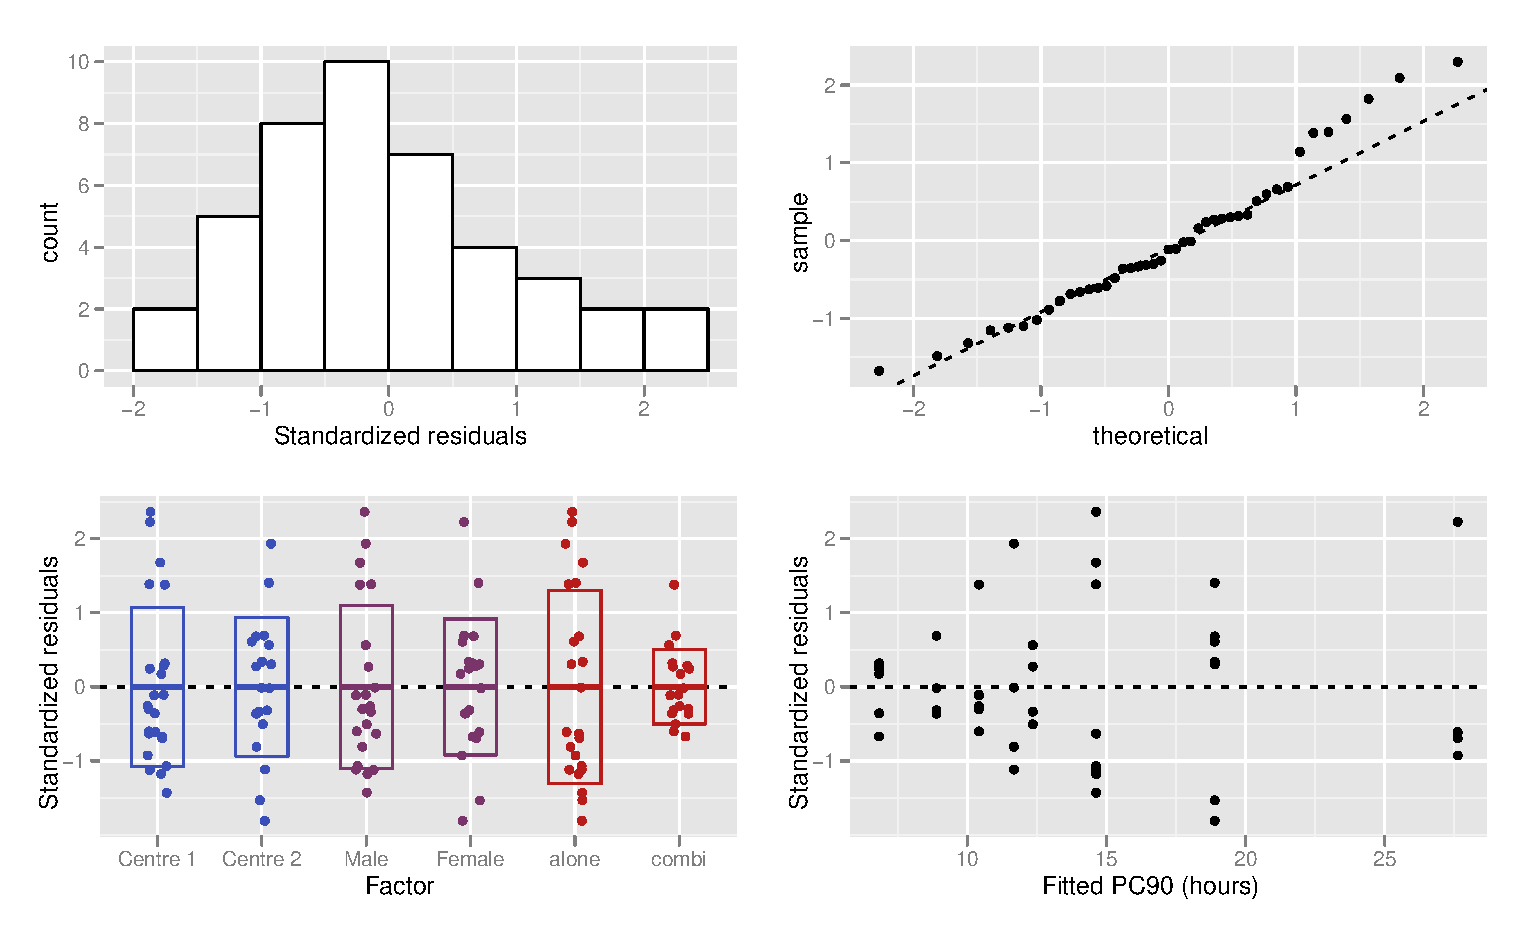
\includegraphics[width=6.5in]{aovloglinres.eps} 
\caption{Residuals from fitting a 3-way ANOVA model with interactions to PC90}
\label{aovloglinres}
\end{figure}
It can be seen that the residuals are approximately normally distributed, but perhaps slightly right skewed. In the plot of the residuals by experimental factor (bottom-left) the standard deviation of the residuals is shown, which when they are standardized, should be approximately 1 and independent of factor. We can see that this is so for centre and sex, but there is heteroscedasticity between treatments with the residuals for the single-drug treatment showing a larger variance than for the combined-drug treatment. We can also see that the variance of the residuals increases with fitted PC90 value (bottom-right).
\begin{table}[h]
\centering
\caption{ANOVA comparison of PC90 estimated by 3 methods}\label{pc90aov}
\begin{tabular}{l|rrrrrl}
Source&Sum Sq.&df&Mean Sq.&$F$&P($>F$)\\
\hline
$Centre$     &               0.1  &1&   0.1 & 0.001 &0.974&\\
$Sex$        &              78.0 &1&   78.0 & 0.813 &0.373&\\
$Treatment$  &            748.2 &1&  748.2 & 7.80 &0.008& **\\
$Centre\times Sex$ &              7.3  &1&   7.3 & 0.077& 0.784&\\
$Centre\times Treatment$ &        84.1 &1&   84.1 & 0.877& 0.356&\\
$Sex\times Treatment$     &     493.8 &1&  493.8 & 5.15 &0.030& *\\
$Centre\times Sex\times Treatment$ &    21.8 &1&   21.8&  0.227& 0.637&\\
$Residuals$      &    3356.4  & 35 & 95.9&&&\\
\hline
Total&4789.7&42&&&
\end{tabular}
$*<0.05\quad**<0.01$
\end{table}

\subsection{ANCOVA}